\documentclass[12pt]{article}
\usepackage{amsmath}
\usepackage{amsfonts}
\usepackage{amsthm}
\usepackage{mathtools}
\usepackage{setspace}
\usepackage{amssymb}
\usepackage{enumerate}
\usepackage{gensymb}
\usepackage{graphicx}
\graphicspath{ {./images/} }
\setcounter{section}{-1}

\renewcommand{\theenumi}{(\alph{enumi})}
\renewcommand{\labelenumi}{\theenumi}
\renewcommand{\phi}{\varphi}

\theoremstyle{definition}
\newtheorem{problem}{Problem}
\newtheorem{solution}{Solution}

\begin{document}
\begin{onehalfspacing}
\noindent{\bf CS440 \hfill Project 1 \hfill Jonathan Delin, Daniel Wang}
\medskip\hrule

\begin{section}{Setup Your Environments}
We created a simple maze environment by randomly assigning each cell to either be unblocked (0) or blocked (1) using weighted probabilities. The following figure is an example of a grid world we generated.\\
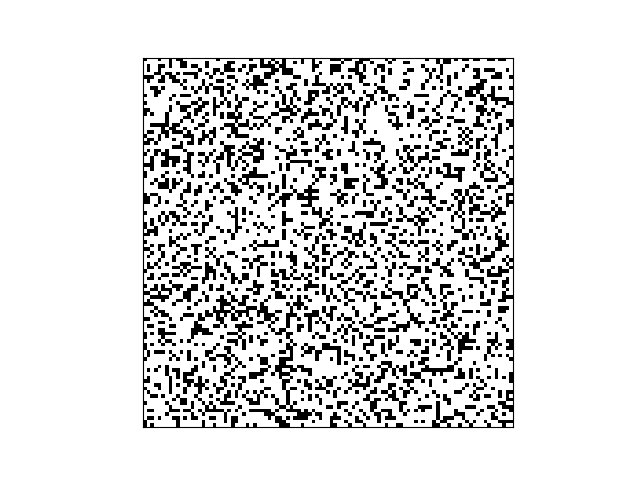
\includegraphics[scale=1]{images/maze00.png}
\end{section}


\begin{section}{Understanding the Methods}
\begin{enumerate}
    \item The first move of the agent for the example search is to the east rather than north because it gives us a smaller heuristic. The Manhattan distance from E3 to T is 2, whereas the Manhattan distance from D2 to T is 4. Since they both have a cost of 1, the f value for E3 is smaller. It is not until the agent actually traverses to the E3 cell that it becomes aware that there is a wall located at E4, at which point it will run another A* search.
    In a finite grid world, there are a finite number of cells. Furthermore, if we do not consider blocked cells, every cell is reachable from any other cell. However, because of blocked cells, we divide the finite grid world into smaller finite regions, where each cell in a given region can access every other cell in that region. When running any A* search, a closed list of expanded cells is kept, so no cell can be expanded twice. Therefore, in a given A* search, every cell in the same region as the agent will eventually be expanded if the target is not reached. If the agent and the target are in the same region, then the agent will find the path to the target in finite time. If the agent and the target are not in the same region, then the agent will expand the finite number of unblocked cells in its region and discover it is impossible to reach the target.\\[1em]
    The way Repeated A* works is that the blocked cells are slowly discovered after every iteration of A*. Every iteration will end in either blocked cells being discovered or the target being reached. Since there are finite number of blocked cells in a finite grid world, all the blocked cells surrounding the region the agent is in will be discovered in finite time, and thus the extent of the region the agent is in will be known, and thus, by the above logic, the agent will either reach the target or discover that it is impossible in finite time.
        

    \item \begin{proof}
    We know that the total number of moves the agent will make is equal to the total number of times A* is called (call it t) multiplied by the total number of moves for each A* call (call it m). Each time A* is called, it moves to a new unblocked cell. Therefore, the number of times A* is called is bounded above by the total number of unblocked cells. Furthermore, since A* never expands a given cell twice, so the number of moves it makes in each A* call is bounded above the total number of unblocked cells. \\[0.5em]
    Thus, if the number of unblocked cells is $n$, we know that $t\leq n$ and $m\leq n$, so $t\times m \leq n\times n$, as desired
    \end{proof}
    

\end{enumerate}

\end{section}

\begin{section}{The Effects of Ties}
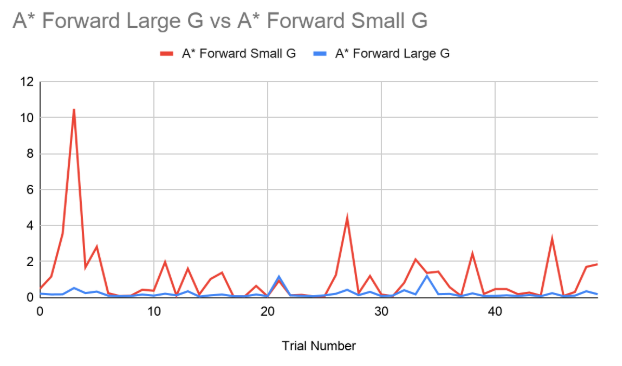
\includegraphics[scale=.8]{images/Tiebreaker Experiment.png}\\
The above chart shows our data for comparing a tiebreaker which favors large g-values with a tiebreaker which favors small $g$-values. We used runtime in seconds as a measurement. The red line represents the tiebreaker which favors a smaller g-value and is consistently greater than the tiebreaker which favors a larger g-value.\\[0.5em]
The reason behind this can be seen by looking at the following figure. If Repeated Forward A* favors a smaller $g$-values value then it will expand the diagonal cells in order, given that there are no obstacles in the grid like in Figure 9. If a larger $g$-values is favored then it will expand cells in the order of how it would traverse using the Manhattan Distance. In the case of an unblocked grid such as Figure 9, the larger $g$-values favor works out better because it will expand less nodes as opposed to smaller $g$-values value which will expand each single one. A larger $g$-values would be much faster for Repeated Forward A* as opposed to a smaller $g$-values favor which will expand much more nodes. \\
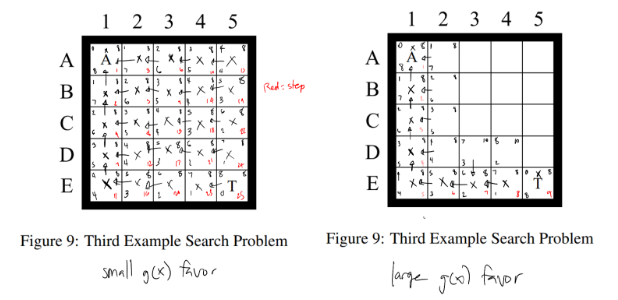
\includegraphics[scale=0.85]{images/Tiebreaker Diagram.png}

\begin{figure}[h]
\caption{Example of A*Forward Small G Path vs A*Forward Large G Path}
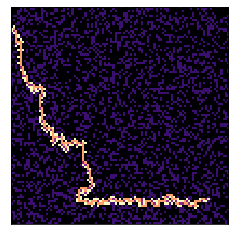
\includegraphics[scale=.8]{images/ForwardLarge.png}
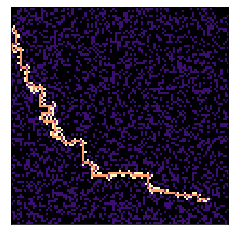
\includegraphics[scale=.8]{images/ForwardSmall.png}
The images above show the difference of using either a small $g$-value or large $g$-value tiebreaker. A small $g$-value tiebreaker expands more cells on average than a large $g$-value tiebreaker. 
\end{figure}




\end{section}

\begin{section}{Forward vs. Backward}
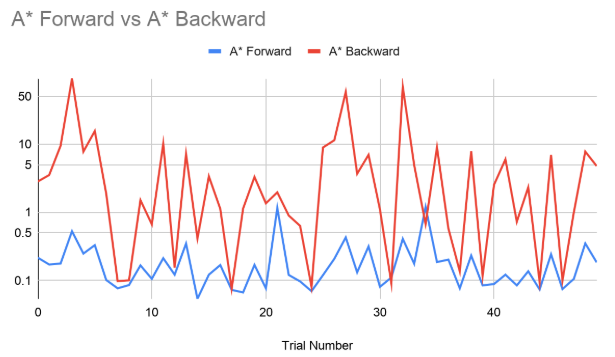
\includegraphics[scale=0.9]{images/Forward vs Backward Experiment.png}
The above chart shows our data for comparing Repeated Forward A* and Repeated Backward A*. The chart compares them using runtime in log(seconds). We used logarithms because the Repeated Backward A* was consistently significantly slower than Repeated Forward A*. We could explain Repeated Backward A*'s slower run speed as a result of it having to re-expand many more nodes whenever it encounters a wall on its journey to finding a path to the start node. If we are starting the A* search near the start point, then we can begin to formulate a path around them much faster than if the A* search started near the goal point. \\
\begin{center}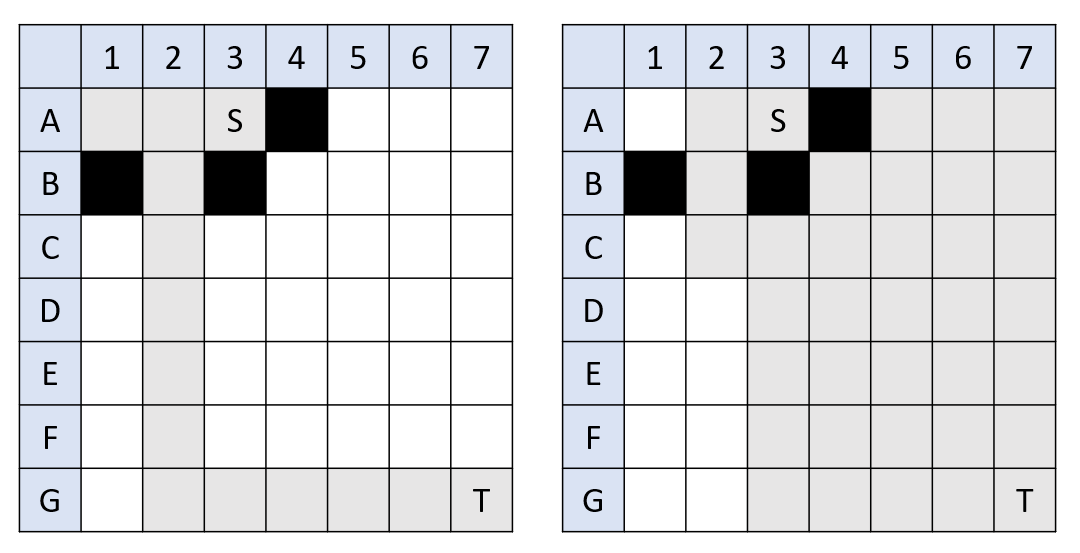
\includegraphics[scale=.4]{images/Forward vs Backward Diagram.png}\end{center}
\noindent{. \hfill Forward A* \hfill Backward A*\hfill .}\\
In the diagram above, the nodes that Forward A* will expand is shown on the left while the nodes that Backward A* will expand is shown on the right. Forward A* will expand way less nodes than Backward A* because it will see the blocked cells first as opposed to Backward A* that will expand many nodes on its initial path based on the Manhattan Distance. Backward A* will start expanding from its position at G7 going upwards all the way to A7 and then expand more nodes going left until it expands A5 and realizes that there is a wall at A4. It will then start expanding from B6 until it reaches and expands B4 where it sees a wall again at B3. Backward A* will then try to expand C6, and once it expands C3, it will see that  C2 has a higher $f$-value, leading it to expand every node that remains not expanded from columns 3 to 7 because they will all have a smaller f-value (actually having an $f$-value of 10 based on the Manhattan Distance where they all just don't account for the blocked cells on the way to the start node) than anything in column 2. Finally, it will expand C2 and find a viable path that will lead it to A3 where the start node is located.\\[0.5em]
Now if a Backward A* was performed on a grid of 101 x 101 cells with many more blocked cells as the project requires, it is no wonder that it will perform significantly worse than Forward A* in most occasions.

\begin{figure}[h]
\caption{Example of A*Forward Large G Path vs A*Backward Large G Path}
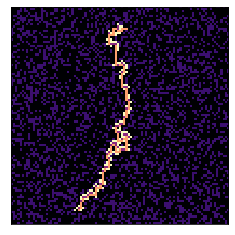
\includegraphics[scale=.8]{images/Forwards1.png}
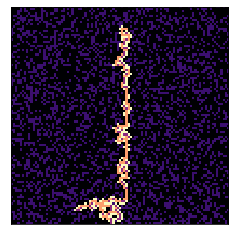
\includegraphics[scale=.8]{images/Backwards1.png}
The images above show the different paths taken by A*Forward and A*Backward.
\end{figure}

\end{section}

\begin{section}{Heuristics in the Adaptive A*}
\begin{proof}
To prove that Manhattan distances are consistent in grid worlds in which the agent can move only in four main conditions we must define a couple of things:
A consistent heuristic is heuristic such that:
\begin{equation*}
    h(s) \leq c(s,a,s') + h(s')
\end{equation*}
and
\begin{equation*}
    h(g) = 0
\end{equation*}
where $s$ is the parent node and $c(s,a,s')$ is the action cost of travelling from node $s$ to node $s'$.\\[0.5em]
The Manhattan Distance formula is:
\begin{equation*}
    h(s) = |X_s - X_{sgoal}| + |Y_s - Y_{sgoal}|
\end{equation*}
where $X$ denotes the index of the rows, $Y$ is the index of the columns, $s$ is the current state of the agent, and $sgoal$ is the goal state. We first consider when $s=sgoal$. In this case, $h(s) = |X_{sgoal} - X_{sgoal}| + |Y_{sgoal} - Y_{sgoal}|=0$, which aligns with our definition of a consistent heuristic. Next, we consider an arbitrary $s$. Suppose $s$ and $s'$ are neighboring cells in the grid world. Thus, we know that
\begin{equation*}
    h(s)-h(s')= (|X_s - X_{sgoal}| + |Y_s - Y_{sgoal}|) - (|X_{s'} - X_{sgoal}| + |Y_{s'} - Y_{sgoal}|)
\end{equation*}
Since, $s$ and $s'$ are directly, adjacent, we know that either $X_s=X_{s'}$ or $Y_s=Y_{s'}$ (but not both). Without loss of generality, assume that $X_s=X_{s'}$, so $|Y_s-Y_{s'}| = 1$ because the two cells are directly adjacent. Thus, 
\begin{equation*}
    h(s)-h(s')= |Y_s - Y_{sgoal}| - |Y_{s'} - Y_{sgoal}| \leq |Y_s - Y_{sgoal} - Y_{s'} + Y_{sgoal}|
\end{equation*}
\begin{equation*}
    =|Y_s - Y_{s'}| = 1 = c(s,a,s')
\end{equation*}
Which means that $h(s)\leq h(s')+c(s,a,s')$, as desired.
\end{proof}
\begin{proof}
Next it is time to address the Adaptive Heuristics. The Adaptive A* updates heuristics based on the previous A* search. The new heuristic is generated by the following formula:
\begin{equation*}
    h_{new}(s) = g(sgoal) - g(s)
\end{equation*}
Where the $g-values$ are from the previous iteration of A*. We know that by definition of $h_{new}$, $h_{new}(sgoal) = g(sgoal) - g(sgoal) = 0$ which satisfies one of the requirements of a consistent heuristic. In order to address the other condition, we proceed by cases. \\[0.5em]
\textbf{Case 1:} $s$ and $s'$ have both been expanded in the previous A* search. \\
By definition of $h_{new}$ we know that
\begin{equation*}
    h_{new}(s) = g(sgoal) - g(s)
\end{equation*}
\begin{equation*}
    h_{new}(s) = g(sgoal) - g(s')
\end{equation*}
We also know that $g(s’) - g(s) \leq c(s, a, s’)$. This statement is true because the two nodes are adjacent and the action cost between them is 1 which is the smallest possible action cost between any two arbitrary nodes in the grid world. Therefore, any A* search which expands both of these nodes will likely expand one as the parent of the other, in which case the difference of their path costs would be 1. If they were not parents, then their path costs would not differ by more than 1 because otherwise being each others parent would have a lower path cost. We now manipulate this statement. First we subtract $g(s')$ from both sides:
\begin{equation*}
    -g(s) \leq -g(s') + c(s, a, s’)
\end{equation*}
Then we add $g(sgoal)$ to both sides:
\begin{equation*}
    g(sgoal)-g(s) \leq g(sgoal)-g(s') + c(s, a, s’)
\end{equation*}
We can then substitute using the equations for $hnew(s)$ and $hnew(s’)$ we defined earlier
\begin{equation*}
    hnew(s) \leq hnew(s’) + c(s, a, s’)
\end{equation*}
which satisfied the definition of a consistent heuristic, as desired. \\[0.5em]
\textbf{Case 2:} $s$ had been expanded in the previous A* but $s'$ had not.\\
We know that 
\begin{equation*}
    h_new(s) = g(Sgoal) - g(s)
\end{equation*}
and $h(s')$ is the Manhattan distance from it to the goal. \\
We know that $s'$ was visited in the previous A* search because it is adjacent to a node which was expanded, namely $s$. Since it was visited but not expanded, its $f$-value must be greater than or equal to the $f$-value of any node which was expanded in the previous search (because A* prioritizes the expansion of smaller $f$-values). We also know that $h(sgoal) = 0$ (which we proved above), so $f(sgoal) = g(sgoal) + 0 = g(sgoal)$. Since $sgoal$ was expanded in the previous search, we know that $f(s’) \geq f(sgoal)$, and thus $f(s') \geq g(sgoal)$. Using the same logic from case 1, we also know that $-g(s) \leq -g(s’) + c(s, a, s’),$ so we can add these two inequalities together to yield
\begin{equation*}
    g(sgoal) - g(s) \leq f(s’) - g(s’) + c(s, a, s’)
\end{equation*}
By definition of $f$-value, $f(s’) = g(s’) + h(s’)$, so $h(s’) = f(s’) - g(s’)$. We substitute to get
\begin{equation*}
    g(sgoal) - g(s) \leq h(s’) + c(s, a, s')
\end{equation*}
By definition of $h_{new}(s)$, $h_{new}(s) = g(sgoal) -g(s)$, so we substitute to get
\begin{equation*}
    h_{new}(s)\leq h(s’) + c(s, a, s’)
\end{equation*}
which satisfies the definition of a consistent heuristic, as desired.\\[0.5em]
\textbf{Case 3:} Neither $s$ nor $s'$ have been expanded previously\\
This will not use the new heuristic because it has not been expanded and the grid has stayed the same or no solution was found. It will still use the old heuristic based on the Manhattan Distance which we have proved is consistent. \\[1em]
These three cases are sufficient to prove that the heuristics in the adaptive A* are consistent, as desired.
\end{proof}
\end{section}

\begin{section}{Heuristics in the Adaptive A*}

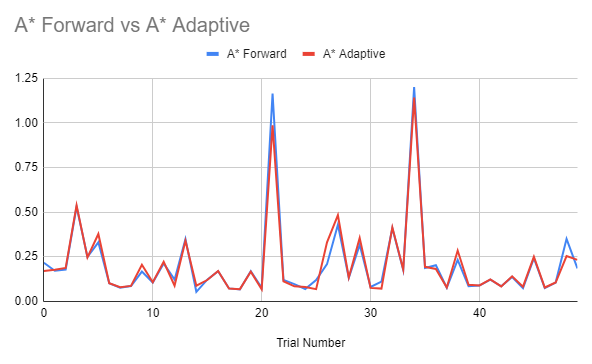
\includegraphics[scale=0.9]{images/Adaptive Experiment.png}

The above chart shows our data for comparing Repeated Forward A* and Adaptive A*. The chart compares them using run time in seconds. The two implementations ran in extremely similar times, with Adaptive A* having the slight edge in a few cases (especially the two times when the run time was over a second). With data so similar, we suspect that some of the fluctuations may also have been due to simply the CPU's memory usage at a particular moment. We also noticed that more often than not, Adaptive A* would run ComputePath fewer times than Forward A*, but we suspect that because of the additional for loop that Adaptive A* uses to update the heuristics, even though the algorithm may be more efficient the run time may have been slightly increased due to this additional requirement. \\[0.5em]
The reason that Adaptive A* is slightly faster is because after each time it runs ComputePath,  the heuristics of all the cells that were expanded are updated to a more accurate, but still increased heuristic. Rather than using the Manhattan distance as the heuristic, the program uses the distance it would have taken for the agent to get to the goal from the cell given its current knowledge of the blocked cells. For example if there is a cell which is at the end of a long ``corridor" then the only possible path from the cell to the goal may not be the simple Manhattan distance, but rather would likely involve exiting through the long corridor. Therefore, the new heuristic would take that lengthy exit into account, and it would be far less likely for the A* search to attempt going down the corridor. The reason that Adaptive A* may not be as effective for us is because the grid worlds we generated had random blocked cells, meaning fewer walls and blocked off sections and more mini obstacles the agent would need to work around.

\begin{figure}[h]
\caption{Example of A*Forward Path vs Adaptive A*Forward Path}
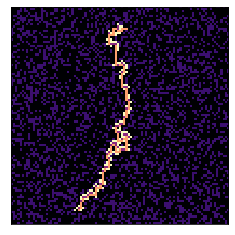
\includegraphics[scale=.5]{images/Forwards1.png}
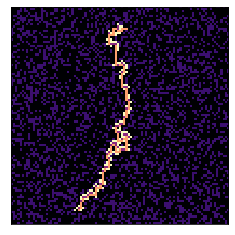
\includegraphics[scale=.5]{images/Adaptive1.png}\\
The images above show the paths taken by A*Forward and Adaptive A* Forward when using a large $g$-value tiebreaker. They have extremely similar paths.
\end{figure}

\end{section}


\begin{section}{Memory Issues}
So in order to reduce memory consumption, we could theoretically minimize the amount of data which needs to be stored per cell. Our implementation stores a lot of data in each cell in order to make the code simpler, but in order to conduct an A* search, we really only need a $g$-value, an $h$-value, a parent indicator, and a search value (which is needed to maintain a level of efficiency in the A* search). Therefore, we should minimize the size of each of these pieces of data. The parent indicator only needs to be 2 bits, because there are only 4 directions the parent could be in. For the other 3 values, they are all bounded above by the number of cells in the gridworld, so we can store them as data points which are $\log_2(w)$ rounded up bits long, where $w$ is the number of cells in the grid world. \\[1em]
When considering a $1001\times 1001$ grid world, there are 1002001 cells. $\log_2(w)$ rounds up to 20, so our three values can each be 20 bits, thus we need 62 bits for each cell. 
\begin{center}
    62 bits $\times$ 1002001 = 62124062 bits = 7.7765507.75 Bytes = 7.766 MB 
\end{center}
If we are limited by 4MB (32 million bits) we must assess how many cells we could handle. The size of a cell could be found using the equation 
\begin{equation*}
    w(3\log_2{w} + 2) \leq 3.2e7
\end{equation*}
This inequality results in a maximal whole number $w$ of $w = 541118$ However, we must round down to one below the nearest power of 2 because we look for the ceiling of the $\log_2(w)$, so we get $2^{19}=524288$.
Thus, with 4MB we can handle a grid world that contains 524,287 cells.


\end{section}

\end{onehalfspacing}
\end{document}